\section{Imitation Learning of An Undelayed Policy}

The idea, as represented in \Cref{fig:imitation_delay_explanation}, is to imitate the policy that an undelayed expert would apply to the current unobserved state.
Since the current state is unknown, only a belief over it can be computed given the augmented state.
Therefore, the delayed policy learns to replicate the action of the undelayed policy under the belief distribution.
We use \textsc{DAgger}~\cite{ross2011reduction} as the imitation learning algorithm, since it is able to account for the shift in distribution between the expert and the learner policies, as explained in \Cref{subsec:imitation_learning}.
This is an important property as the shift in state distribution is being exacerbated by the delay. 
This shift will be discussed in greater detail in \Cref{subsec:analysis_ismmdp}.

\begin{figure}[t]
    \centering
    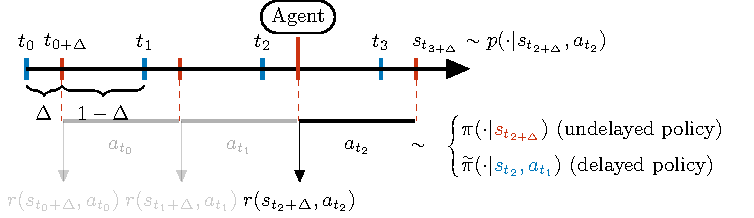
\includegraphics[labelimitation=dualitytrajectory]{img/thesis_plots_imitation.pdf}
    \caption{Representation of the imitation of an undelayed policy $\pi$ (expert) by a delayed policy $\delayedpolicy$ (learner).
    The latter tries to replicate the actions of the former seeing only the augmented state and is blind to the current state $s_t$.}
    \label{fig:imitation_delay_explanation}
\end{figure}


\subsection{Duality of Trajectories}
An important prerequisite for the application of \textsc{DAgger} is the ability of both the expert and the learner to sample from the environment.
This is possible for constantly delayed \gls{dmdp} thanks to what we call the \emph{duality of trajectories}.
On the one hand, in an \gls{mdp}, a \emph{synthetic} augmented state can be created by ignoring the most recent state information and providing the agent with a past state and the sequence of action taken since then. 
In this way, it is possible to sample from a delayed policy in an undelayed environment.
On the other hand, an agent in a delayed environment will eventually observe its current state\footnote{This does not generally occur in a POMDP.}. 
Thanks to this property, the probability of any trajectory sampled with a delayed policy can be computed under an undelayed policy.
All things considered, once sampled, a trajectory can be studied both from the point of view of a delayed or an undelayed policy, regardless of how this trajectory was sampled.
Therefore, the constantly delayed \gls{dmdp} satisfies the prerequisite to apply \textsc{DAgger} to our imitation problem.


\subsection{Delayed Imitation with
Dataset Aggregation (DIDA)}
\label{subsec:dida_algo}

\subsubsection{General Algorithm}
Following the framework of \textsc{DAgger} (see~\Cref{subsec:imitation_learning}), we propose Delayed Imitation with Dataset Aggregation (DIDA). 
As \textsc{DAgger}, DIDA samples from the environment by following either the expert or learner policy.
If the expert is chosen, then our undelayed policy $\pi$ is queried on the current state of the environment. Instead, if the learner policy is chosen, an augmented state is synthetically built from the history of the trajectory and fed to the delayed policy $\delayedpolicy$. 
In practice, this means that a buffer of the recent history must be maintained. 
For the imitation step, DIDA builds a dataset $\mathcal{D}=(x^{(i)},a_E^{(i)})_{0\le i\le N}$ of tuples of augmented states $x^{(i)}$ and actions $a_E^{(i)}$ selected by the undelayed policy at the current unobserved state. 
The delayed policy is then trained on $\mathcal{D}$ to replicate the expert's actions given an augmented state.
A practical remark is that the storage of the augmented states can be made efficiently. 
In fact, most actions in two consecutive augmented states are the same. 
It, therefore, suffices to store state-action histories and build the augmented states only at training time. 
We provide the algorithm for DIDA in \Cref{algo:dida}.


\subsubsection{DIDA Without Undelayed Environment}
\label{subsubsec:dida_no_undelayed_env}
Should one not have access to an undelayed environment where DIDA can be applied straightforwardly, a little modification to the algorithm allows it to be used anyway. 
When the undelayed policy should have been queried on the unobserved current state, it is instead possible to query the undelayed policy on the last observed state, that is, in a memoryless fashion (see~\Cref{subsec:memoryless}). 
This is even more relevant when the $\beta$-routine of \textsc{DAgger} satisfies $\beta_1=1, \beta_{i\ge 2}=0$ (see~\Cref{subsec:dida_algo}). 
That is, only the first iteration is made with the undelayed policy (when the delayed policy has not been trained yet), and successive ones query only the delayed policy.
Two modifications should be made to \Cref{algo:dida}.
First, in Line 5, we substitute $a_E\sim\pi(\cdot\vert s_{1})$ for $a_E\sim\pi(\cdot\vert s_{\delay+1})$.
Second, the population of the dataset $\mathcal{D}$ should be changed. 
Indeed, we are not interested in the actions selected in a memoryless fashion by the expert. 
Instead, the actions of the expert stored in $\mathcal{D}$ should correspond to the action selected by the expert in the unobserved current state. 
This implies that, in practice, observing an augmented state $x$, the agent has to wait for $\delay$ steps to observe the current unobserved.
Only then can the memoryless expert provide the action $a_E$ to be added together with $x$ to the dataset $\mathcal{D}$. 
Therefore, line 10 of \Cref{algo:dida} must be delayed accordingly.
We refer to this variant of DIDA as memoryless-DIDA (M-DIDA).


\subsubsection{Policy Learnt by DIDA}
In stochastic \glspl{mdp}, the support of the belief for the unobserved current state may expand over many states. DIDA will learn to replicate the expert's actions under this distribution. 
Formally, DIDA's output policy under perfect imitation is as follows: 
\begin{align}
    \delayedpolicy(a\vert x) = \int_{\statespace} \augmentedbelief(s\vert x) \pi(a\vert s)\de s.\label{eq:belief_pol}
\end{align}
Notably, this policy can be seen as a model-based one and  \Cref{pp:counter_example_belief_based} applies to it. Therefore there exists \glspl{mdp} where DIDA is sub-optimal compared to the best-undelayed policy. We will see in the theoretical analysis in \Cref{sec:th_analysis_imitation} that this policy is however efficient in smooth \glspl{mdp}.

The policy in \Cref{eq:belief_pol} is obtained under perfect imitation, in practice however, depending on the loss function, this policy might be different. We give two examples below.

\noindent\textbf{Mean squared error loss.}\indent For $x$ sampled from $\mathcal{D}$, if the imitation step of DIDA satisfies,
\begin{align*}
    \argmin_{\vectorialform{\theta}\in\Theta} \int_{\statespace}\int_{\actionspace} (a-\delayedpolicy_{\vectorialform{\theta}}(x))^2 \pi(a\vert s) \augmentedbelief(s\vert x)\de a\de s,
\end{align*}
then, the policy it will output is,
\begin{align*}
    \delayedpolicy_{\vectorialform{\theta}^\star}(x) = \expectedvalue_{s\sim \augmentedbelief(\cdot\vert x)}\left[ \expectedvalue_{a \sim\pi(\cdot \vert s)}[a]\right].
\end{align*}
That is, the policy returns the mean value of the expert policy over the belief. 

\noindent\textbf{Kullback-Leibler loss.}\indent For $x$ sampled from $\mathcal{D}$, the policy learnt by DIDA will satisfy:
\begin{align}
    &\argmin_{\vectorialform{\theta}\in\Theta} \int_{\statespace} \kullbackleiblerdivergence(\pi(\cdot \vert s) \Vert \delayedpolicy_{\vectorialform{\theta}}(\cdot \vert x)) \augmentedbelief(s\vert x)\de s\nonumber
    %\\
    %&= \argmin_{\theta} \int_{\statespace} \int_{\actionspace} \pi(a \vert s) \log \pi(a \vert x)) b(s\vert x)~da~ds - \int_{\statespace} \int_{\actionspace} \pi(a \vert s) \log \delayedpolicy_{\vectorialform{\theta}}(a \vert x)) \augmentedbelief(s\vert x)~da~ds\nonumber
    \\
    &= \argmin_{\vectorialform{\theta}\in\Theta} - \int_{\statespace} \int_{\actionspace} \pi(a \vert s) \log \delayedpolicy_{\vectorialform{\theta}}(a \vert x)) \augmentedbelief(s\vert x)\de a \de s\label{eq:indpt_theta}
    \\
    &= \argmin_{\vectorialform{\theta}\in\Theta}  - \int_{\actionspace}\int_{\statespace}  \pi(a \vert s) \log \delayedpolicy_{\vectorialform{\theta}}(a \vert x)) \augmentedbelief(s\vert x)\de s \de a\label{eq:fubini}
    \\
    &= \argmin_{\vectorialform{\theta}\in\Theta}  \int_{\actionspace} \int_{\statespace}  \pi(a \vert s) \augmentedbelief(s\vert x)\log\left(\augmentedbelief(s\vert x) \pi(a \vert x))\right)\de s\de a\nonumber
    \\
    &\qquad- \int_{\actionspace}\int_{\statespace}  \pi(a \vert s) \log \delayedpolicy_{\vectorialform{\theta}}(a \vert x)) \augmentedbelief(s\vert x)\de s\de a\label{eq:add_pas_depend_theta}
    \\
    &= \argmin_{\vectorialform{\theta}\in\Theta}  D_{KL}\left(\left.\int_{\statespace}\pi(\cdot \vert s)b(s\vert x)\de s \right\Vert \delayedpolicy_{\vectorialform{\theta}}(\cdot \vert x)\right) ,\nonumber
\end{align}
where \Cref{eq:indpt_theta} holds by expanding the Kullback-Leibler distance and noticing that one term does not depend on $\vectorialform{\theta}$; \Cref{eq:fubini} holds by Fubini's theorem since the functions inside the integral are always negative; \Cref{eq:add_pas_depend_theta} is obtained by adding a term which does not depend on $\vectorialform{\theta}$.



\begin{algorithm}[t] 
\caption{Delayed Imitation with \textsc{DAgger} (DIDA)}\label{algo:dida}
\textbf{Inputs}
(un)delayed \gls{mdp} $\markovdecisionprocess$, undelayed expert $\pi$, $\beta$-routine, number of steps $N$, empty dataset $\mathcal{D}$.\\
\textbf{Outputs}: delayed policy $\delayedpolicy$
\begin{algorithmic}[1]
    \FOR{$\beta_i$ in $\beta$-routine}%\{$1,\dots,N$\}}
        \FOR{$j$ in $\{1,\dots,N\}$}
            \IF{New episode}
                \STATE Initialize state buffer $( s_{1},s_{2}, \dots, s_{\delay+1})$ and action buffer $( a_{1},a_{2} \dots, a_{\delay})$
            \ENDIF
            \STATE Sample $a_E\sim\pi(\cdot\vert {{s}}_{\delay+1})$, set $a=a_E$ \label{ope:undelayed_sample}
            \IF{Random $u \sim U([0,1])\geq \beta_i$}
                \STATE Overwrite ${ a \sim\pi_I(\cdot\vert [{s}_{1},a_{1}, \dots, a_{\delay}])}$ 
            \ENDIF
            \STATE Aggregate dataset:
            $$\qquad \mathcal{D}\gets \mathcal{D} \cup ([{s}_{1}, a_{1}, \dots, a_{\delay}],a_E)$$
            \STATE Apply $a$ in $\markovdecisionprocess$ and get new state $s$ 
            \STATE Update buffers:
            $$\qquad ({s}_1,\dots,{s}_{\delay+1}) \gets ({s}_2,\dots,{s}_{\delay+1},s)$$
            $$\qquad  ({a}_1,\dots,{a}_{\delay}) \gets ({a}_2,\dots,{a}_{\delay},a)$$
            \ENDFOR
        \STATE Train $\delayedpolicy$ on $\mathcal{D}$ 
    \ENDFOR
\end{algorithmic}
\end{algorithm}


\subsection{Non-integer Delays}
\label{subsec:dida_non_int}
We will now extend the previous algorithm to the non-integer delay case. 
However, we first need to derive some theoretical results that allow us to extend the framework. 


\subsubsection{Theory of Non-integer Delays}
Observe that, even for a delay smaller than one step $\delay\in (0,1)$, an augmented state $x_t = (s_t,a_{t-1})\in \statespace \times \actionspace \eqqcolon \augmentedstatespace$ is necessary.
This follows from the observation that the action applied at some time $t+\epsilon$, where $\epsilon\le\delay$ is still the action $a_{t-1}$ selected at the previous step. 
In the remainder of this thesis, we use the notation "~$\integerpart{\ }$~" for the integer part of a real number, "~$\fractionalpart{\ }$~"  for its fractional part and "~$\lceil\ \rceil$~" for the smallest integer greater than it. 
For the construction of the non-integer delayed environment from two interleaved \glspl{mdp}, refer to \Cref{subsec:non_int_delays}. 
When $\delay\in (0,1)$, those interleaved \glspl{mdp} are $\markovdecisionprocess$ and $\markovdecisionprocess_\delay$. 
Instead, when $\delay>1$, we only need to shift the second \gls{mdp} of the fractional part of the delay. The two \glspl{mdp} therefore are $\markovdecisionprocess$ and $\markovdecisionprocess_{\fractionalpart\delay}$. 
Our first result is that the problem of non-integer delay can be cast back to an \gls{mdp}. 

\begin{prop}
\label{pp:equivalent_mdp_non_int}
    Let $\delay\in\realnumbers[\ge0]$ be a (non-)integer delay, and consider a \gls{dmdp} $\delayedmarkovdecisionprocess$, constantly delayed by $\delay$ in its action execution or state observation.  
    The problem can then be cast back into an \gls{mdp} by augmenting the state with the last $\lceil\delay\rceil$ actions.
\end{prop}
\begin{proof}
    We prove this result for the action execution delay but the proof for state observation follows parallel considerations. 
    We construct an \gls{mdp} $\markovdecisionprocess$ using the augmented state space $\augmentedstatespace=\statespace\times\actionspace^{\lceil\delay\rceil}$ as its state space such that, for any delayed policy, its return in $\markovdecisionprocess$ is equal to that in $\delayedmarkovdecisionprocess$.
    For augmented states $x=(s,a_1,\dots,a_{\lceil\delay\rceil})$ and $x'=(s',a_1',\dots,a_{\lceil\delay\rceil}')$ in $\augmentedstatespace$, the new transition distribution reads
    \begin{align*}
        \augmentedtransitionfunction(x'\vert x, a)\coloneqq 
        p(s'\vert s,a_1)\delta_a(a_{\lceil\delay\rceil}')\prod_{i=1}^{\lceil\delay\rceil-1}\delta_{a_{i+1}}(a_{i}').
    \end{align*}
    Note that, in the case $\delay\notin \naturalnumbers$, $p$ is defined as in \Cref{eq:def_p_non_int}:
    \begin{align}
        p(s'\vert s,a)=\int_{\statespace}   \augmentedbelief[1-\fractionalpart{\delay}](s'\vert z,a)\augmentedbelief[\fractionalpart{\delay}](z|s,a)\de z.
    \end{align}
    Now, for $x=(s,a_1,\dots,a_{\lceil\delay\rceil})$, one defines the expected reward as,
    \begin{align*}
        \augmentedexpectedrewardfunction(x,a) = \expectedvalue_{z\sim \augmentedbelief(z\vert x)}[\expectedrewardfunction(z,a)].
    \end{align*}
    To conclude the proof, let $\delayedpolicy$ be any history-dependent policy for $\delayedmarkovdecisionprocess$. Now, assume that the histories of observed state and action $(s_0,a_0,\dots,s_{t},a_t,\dots,a_{t+\lceil\delay\rceil-1})\in\statespace^t\times\actionspace^{t+\lceil\delay\rceil}$\footnote{The history on $\augmentedstatespace^t\times\actionspace^t$ clearly defines a history on $\statespace^t\times\actionspace^{t+\lceil\delay\rceil}$.} is the same in $\delayedmarkovdecisionprocess$ and $\markovdecisionprocess$ at time $t$. 
    Any agent whose policy is based on the history then selects the next action $a_{t+\lceil\delay\rceil}$ with the same probabilities in $\markovdecisionprocess$ and $\delayedmarkovdecisionprocess$.
    In $\delayedmarkovdecisionprocess$, given its current observed state $s_t$ and the action $a_{t}$ whose effect he has not yet seen, the agent observes a new state $s_{t+1}$ with probability $p(s_{t+1}\vert s_t,a_{t})$. 
    In $\markovdecisionprocess$, the state $s_{t+1}$ contained in the new augmented state is also sampled from $p(s_{t+1}\vert s_t,a_{t})$ by design. 
    Therefore, the histories also match at $t+1$. 
    By recurrence, this holds for any $t'>t$.
    It suffices to initialise the processes in the same manner to have the same state distribution over $\statespace$.
    Having the same histories, the reward collected in 
    $\delayedmarkovdecisionprocess$ and $\markovdecisionprocess$ are also equal by design.
    This means that any delayed policy achieves the same return in both processes.
\end{proof}

Note that to prove the previous proposition for state observation delays, the two \glspl{mdp} $\markovdecisionprocess$ and $\markovdecisionprocess_{\fractionalpart\delay}$ are switched.
In fact, consider $\delay\in(0,1)$; for an action execution delay, the agent sees the current state $s_t$ but its action $a_t$ is executed at $t+\delay$, in state $s_{t+\delay}$. 
In the case of state observation delay, if the agent's current unobserved state was also $s_t$, then the last observed state would be $s_{t-\delay}$, which does not belong to $\markovdecisionprocess_{\delay}$ if $\textstyle\delay\neq \frac{1}{2}$.
Instead, placing the current unobserved state at $s_{t+\delay}$, then the delayed state always belongs to $\markovdecisionprocess$.
To summarize, the difference between the two processes is when the agent selects an action. 
For action execution delays, the agent selects an action while its current state is in $\markovdecisionprocess$ whereas, for state observation delays, the agent selects an action while its current state is in $\markovdecisionprocess_{\delay}$
This shift in control steps can be visually understood in \Cref{fig:non_int_delay_def}.

We now provide a result which shows that, as in the integer case, the action execution and state observation delays are equivalent in the non-integer one. 
\begin{prop}
    Let $\delay\in\realnumbers[\ge0]$ be a (non-)integer delay.
    Let $\markovdecisionprocess$ and $\markovdecisionprocess_{\fractionalpart{\delay}}$ be two interleaved \glspl{mdp} over which we define two constantly-delayed \glspl{dmdp}: $\delayedmarkovdecisionprocess$ is $\delay$-delayed in the action execution and $\delayedmarkovdecisionprocess'$ is $\delay$-delayed in the state observation\footnote{Fixing first $\markovdecisionprocess$ and $\markovdecisionprocess_{\fractionalpart{\delay}}$ ensures that the observed state and the state on which the action is executed correspond in the two \glspl{dmdp}. 
    Otherwise, one could build them such that the action-delayed agent observes $s_t$ and acts on $s_{t+\delay}$ while the state-delayed agent observes $s_{t-\delay}$ and acts on $s_{t}$. There would be a mismatch in this case.}. 
    Then, $\delayedmarkovdecisionprocess$ and $\delayedmarkovdecisionprocess'$ are equivalent.
\end{prop}
\begin{proof}
    The proof follows easily by observing that the equivalent \glspl{mdp} constructed in \Cref{pp:equivalent_mdp_non_int} are the same.
\end{proof}


\subsubsection{DIDA for Non-integer Delays}
\label{subsubsec:dida_non_int}

We are now ready to extend DIDA to the non-integer case. We will use the notations of \Cref{subsec:non_int_delays} for the two interleaved \glspl{mdp} $\markovdecisionprocess$ and $\markovdecisionprocess_\delay$ defining the non-integer delay. 
As in DIDA, the first step is to learn an undelayed policy. Here, the undelayed policy is learnt in $\markovdecisionprocess_\delay$.
The state observed by the delayed agent will instead be that of $\markovdecisionprocess$.
We provide the modified algorithm in \Cref{algo:dida_non_int}.
The main difference from \Cref{algo:dida} is that DIDA must keep in memory the $\lceil\delay\rceil$ last actions. 
Moreover, DIDA must also keep a buffer of the states both from  $\markovdecisionprocess$ and $\markovdecisionprocess_\delay$ as the former will be used for the augmented state and the latter for computing the undelayed expert's actions.
Note that the policy learnt by DIDA for non-integer delays still satisfies \Cref{eq:belief_pol}.

\begin{remark}
    A similar idea could be used for the algorithm presented in the previous section.
    D-TRPO could be adapted to learn a representation of the belief in $\markovdecisionprocess_\delay$ while observing a state in $\markovdecisionprocess$.
\end{remark}


\subsubsection{Time-Lipschitzness for Non-integer Delays}
Finally, in order to expand the theory of the next section, we include non-integer delays in the definition of the $L_T$-TLC~(\Cref{def:time_lip}). Given $\delay\in(0,1)$, a \gls{dmdp} is $L_T$-TLC if $\forall s,a\in \statespace\times\actionspace$,
\begin{align}
\label{eq:time_lip_non_int}
    \wassersteindistance(b_\delay(\cdot\vert s,a), \delta_s)\le \delay L_T.
\end{align}




\begin{algorithm}[t] 
\caption{DIDA for non-integer delays ($\delay\in\realnumbers[\ge0]$)}\label{algo:dida_non_int}
\textbf{Inputs}:
$\{\delay\}\coloneqq\delay-\lfloor\delay\rfloor$, \glspl{mdp} $\markovdecisionprocess$ and $\markovdecisionprocess_{\{\delay\}}$ obtained from continuous-time \gls{mdp}, undelayed expert $\pi$ trained on $\markovdecisionprocess_{\delay}$, $\beta$-routine, number of steps $N$, empty dataset $\mathcal{D}$.\\
\textbf{Outputs}: delayed policy $\pi_I$
\begin{algorithmic}[1]
    \FOR{$\beta_i$ in $\beta$-routine}%\{$1,\dots,N$\}}
        %\State Initialize action queue $ \underline a\leftarrow \emptyset$
        \FOR{$j$ in $\{1,\dots,N\}$}
            \IF{New episode}
                \STATE Initialize state buffer $( s_{1},s_{1+\fractionalpart{\delay}}, \dots, s_{\lceil\delay\rceil},s_{\delay+1})$ and action buffer $( a_{0},a_{1} \dots, a_{\lfloor\delay\rfloor})$
            \ENDIF
            \STATE Sample $a_E\sim\pi(\cdot\vert {{s}}_{\delay+1})$, set $a=a_E$
            \IF{Random $u \sim U([0,1])\geq \beta_i$}
                \STATE Overwrite ${ a \sim\delayedpolicy(\cdot\vert [{s}_{1},a_{0}, \dots, a_{\lfloor\delay\rfloor}])}$ 
                % \State $a \leftarrow a_I$
            \ENDIF
            \STATE Aggregate dataset:
            $$\mathcal{D}\leftarrow \mathcal{D} \cup ([{s}_{1}, a_{0},a_2, \dots, a_{\lfloor\delay\rfloor}],a_E)$$
            \STATE Apply $a$ at $s_{\delay+1}$ and get new states $(s_{\lceil\delay\rceil+1},s_{\delay+2})$
            \STATE Update buffers:
            $$(s_{1}, s_{1+\fractionalpart{\delay}}, \dots, s_{\lceil\delay\rceil},s_{\delay+1}) \leftarrow ( s_{2},s_{2+\fractionalpart{\delay}}, \dots, s_{\lceil\delay\rceil+1},s_{\delay+2})$$
            $$({a}_0,\dots, a_{\lfloor\delay\rfloor}) \leftarrow ({a}_1,\dots,a_{\lfloor\delay\rfloor},a)$$
            \ENDFOR
        \STATE Train $\delayedpolicy$ on $\mathcal{D}$ 
    \ENDFOR
\end{algorithmic}
\end{algorithm} 



\subsection{DIDA for Learning Multiple Delays at Once}
\label{subsubsec:multi_delay_once_imitation}

The same idea as in \Cref{subsec:multi_delay_once_belief} can be applied to DIDA.
A policy learnt for a delay $\delay>0$ can be leveraged to act in an environment with smaller delays $0<\delay'<\delay$ by simulating a delay of $\delay$.
We provide experiments in \Cref{sec:exp_imitation} to illustrate the effectiveness of the idea. 